After installing/compiling \biodeg{} as described in Section~\ref{sec:installation}, we are ready to run it. There are 2 ways to run \biodeg{} simulations: 1) using the UI to configure and execute \biodeg{}, or 2) running \biodeg{} directly from command line and provide simulation parameters via command line arguments. Moreover, in a hybrid approach, the UI can be used to configure and generate the command for method \#2, which can be useful in which you want to configure the simulation only and run it later in another environment like on a super-computer or cluster.

The UI can be run simply by double clicking on the \verb|BioDeg-UI.exe| in Windows or by executing \verb|./BioDeg-UI| in Linux. For running \biodeg{} directly, one need to execute the following command:
\begin{verbatim}
$ mpirun -n N FreeFem++-mpi BioDeg-core/src/main.edp <command line args>
\end{verbatim}
in which N defines the number of MPI processes to be used. The full list of command line arguments can be found in Section \hyperref[sec:index]{Index}.

In order to clarify and demonstrate the procedure of performing simulations using \biodeg{}, 2 step-by-step examples are provided in Section~\ref{sec:config}, showing how to configure and run simulations with and without the UI. The mesh files needed to run these examples can be found in the \verb|demo| directory.

\subsection{Configuring the simulation} \label{sec:config}


\subsubsection{Example 1 - degradation of a simple screw}\label{sec:example1}

Let us consider the first example given in the \verb|demo| directory, where we simulate the biodegradation of a small screw. The size of the screw was chosen to be very small intentionally to make the simulation shorter such that the user can see the effect of the degradation much faster. The input mesh file is named \verb|screw.mesh|. For this example, we use the \biodeg{}-UI interface to perform the simulation. 

Let's conduct the first simulation with most of the parameters left with their default values. Run the user interface, and mark \menu[,]{Geometry \& Mesh, Import external mesh}. Then click the browse button in front of the ``File'' box (\menu[,]{Geometry \& Mesh, Import mesh, File}), navigate to the \verb|demo| directory, and select the \verb|screw.mesh| file. The path should be inserted in the ``File'' box. Selecting appropriate label numbers of the external mesh is very crucial in \biodeg{}, so you should always check the labels before importing the mesh. One of the best tools to do this is GMSH, in which you can view the labels of mesh files by opening the mesh and navigating to \menu[,]{Tools, Visibility}. Doing this on the \verb|screw.mesh| shows that the label number of the scaffold is 2 while the medium has a label number of 1 (Fig.~\ref{fig:gmsh_label}). So, we need to switch the default labels by selecting 2 for the scaffold (\menu[,]{Geometry \& Mesh, Import mesh, Scaffold label}) and 1 for the medium (\menu[,]{Geometry \& Mesh, Import mesh, Medium label}).

\begin{figure}[h]
\center 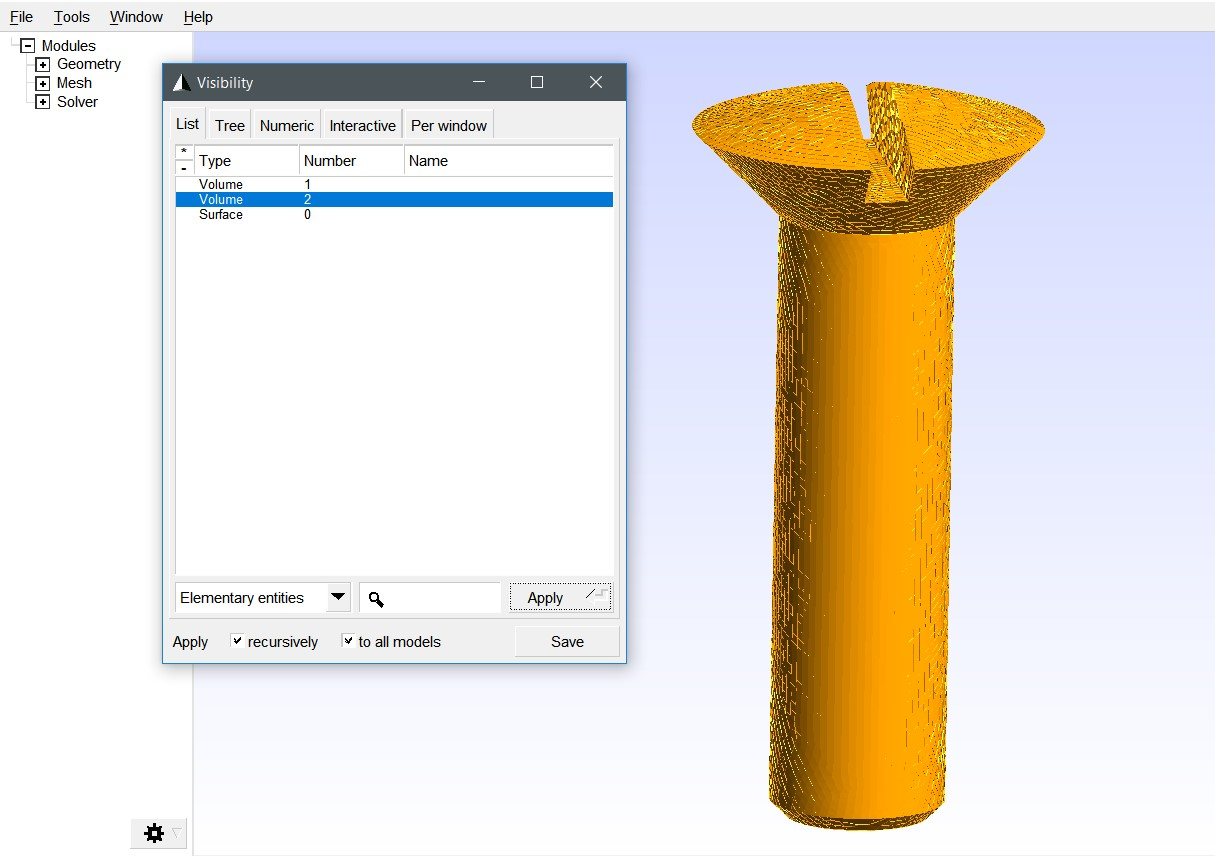
\includegraphics[width=15cm]{gmsh_label}
\caption{Using GMSH to read the labels of the mesh} \label{fig:gmsh_label}
\end{figure}

We need to enable the VTK output if we want to see the graphical output of the simulations. Navigate to \menu[,]{Output, Output options, Write VTK output} and mark it. You should also specify the output directory by clicking on the browse button in front of the ``Output directory'' (\menu[,]{Output, Output options, Output directory}) and select a directory of desire. 

That was all we needed to do to setup a simulation in \biodeg{}, and you can start the simulation by pressing the \menu[,]{Run simulation} button located in the middle of the main window. There are lot more parameters we can deal with (see Section \hyperref[sec:index]{Index}), but the input and output are the most essential ones. 

Although you can start the simulation of this example right now, there is a couple of more things you may want to change:

\begin{itemize}
\item
In \biodeg{}, simulations are by default carried out in parallel using domain decomposition, meaning that the simulation is distributed among available computing nodes. If you are running \biodeg{} on your local machine, you may need to adjust the parallel computing settings. Navigate to \menu[,]{Solver, Parallel computing, Enable parallel computing} and disable it if you don't want to parallelize the simulation. If you want to continue with parallelization enabled (default behavior), you may need to adjust the number of parallel processes to match the number of free CPU cores you have on your machine. You can change it in \menu[,]{Solver, Parallel computing, CPU/MPI cores}. 
\item
The default degradation rate is quite fast, so you may want to decrease it by reducing the diffusion coefficient of the metallic ions (please refer to ``Theory Guide'' if you want to know more about diffusion controls the rate of degradation). The default diffusion rate is the value we have estimated for saline solutions, which leads to a high rate of corrosion. You can apply this it by changing the value in \menu[,]{Material \& BCs, Reaction-diffusion properties, Metal ion diffusion coefficient} and reduce it to something like $0.0005$, which is its order when it comes to buffered solutions and simulated body fluids.
\item
The results write interval, implying how frequently you want to store the results, affects the resource consumption (which is storage in this case) and the quality of the graphical postprocessing. So, you should configure this carefully to keep the balance of the quality and resource consumption. The default save interval is $0.25$ hours of simulation time, but you can change it in \menu[,]{Output, Output options, Save results every ... hours}. For this simulation, since the screw geometry is small and degrades very fast, you can reduce this to $0.1$ to be able to see the degradation steps better.
\item
Final simulation time does not affect the simulation progress, but it is always a good practice to adjust it, enabling us to track the progress of the simulation better and avoid wasting resources (both computing power and storage). The default simulation time is 21 hours, but you can reduce it in \menu[,]{Solver, Time control, Final simulation time (hour)}. For this simulation, you can reduce it to 2.
\end{itemize}

After running the simulation (by pressing the \menu[,]{Run simulation} button), you can view the progress of the simulation on the UI, showing you how many steps have been taken and how much material degradation has happened. The UI also shows you the details info of the size of the problem, including the degrees of freedom (DOF) of each equation and the number of elements, as well as the number of DOFs for each sub-domain after mesh partitioning (for parallel computing). %add a figure showing DOF and progress

Running this simulation leads to the results demonstrated in Fig.~\ref{fig:screw_degradation}, showing how the screw degrades. For more information on how to postprocess the results, please refer to the postporcessing section.

\begin{figure}[h]
\center 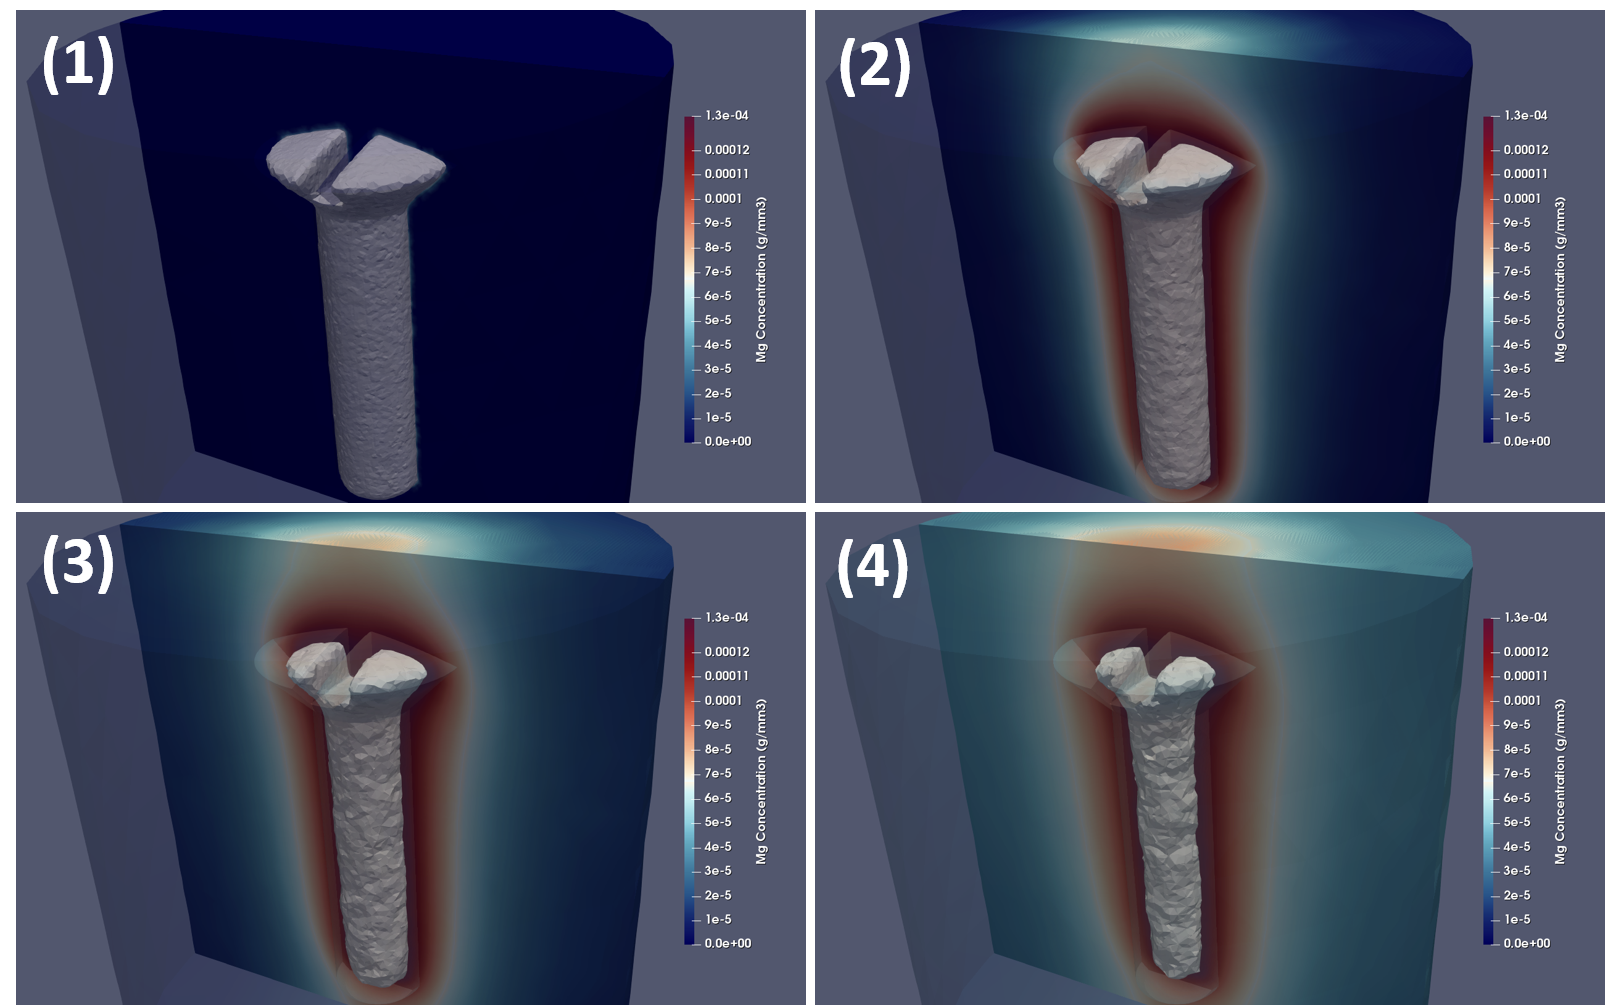
\includegraphics[width=15cm]{screw_degradation}
\caption{Simulation of the biodegradation of a simple screw, showing how the material is released and how the implant degrades.} \label{fig:screw_degradation}
\end{figure}


\subsubsection{Example 2}\label{sec:example2}


